\section{Examples showcasing features of $\lgname$ language and simulator}
\label{sec:experims}
The $\lgname$ simulator provides the user a way to test and  debug application programs with different and heterogeneous physics models. We present three case studies to demonstrate some of the key features of the $\lgname$ language and its  simulator.

\subsection{Platooning}
%end to end
\label{sec:platooning}
Figure~\ref{fig:platooningapp} shows the $\lgname$ program for a simplified platooning protocol for vehicles on a single lane. The position of successive vehicles is communicated through  {\bf allread} shared variable $\mathit{x}$. The  goal is to maintain a minimal  \emph{safe} separation  of $5$ meters between any two consecutive cars. For the sake of simplicity, here the leading car  has a preprogrammed behavior (it sets its acceleration to $2$ or $-2$ every $100$ rounds); in a more realistic deployment this behavior could be based on speed limits or other traffic. 
%The motion controller for the car has bounds on highest and lowest velocities allowed. 
Every other car in the platoon with pid $i$ sets the actuator, namely, its acceleration $\mathit{Motion.xacc}$ based on its distance from the car with pid $i+1$; slowing down when the separation is less than the $\mathit{threshold}$ of $8$ meters, accelerating otherwise. 
%The cars communicate through the \emph{allread} variable $\mathit{pos}$, which they update every time they execute the event \emph{SetAcc}, or, as the semantics dictates, every $\delta$ time units.

\begin{figure}[ht!]
\begin{mdframed}
    \noindent
    \begin{center}
        \scriptsize
        \two{0.4}{0.6}
        {\lstinputlisting[language=koordNums,firstline=1,lastline=14,frame=none]{code/platooning3.tex}}
        {\lstinputlisting[language=koordNums,firstline=15,frame=none,firstnumber=15]{code/platooning3.tex}} 
    \end{center}
\end{mdframed}
    \caption{$\lgname$ program for robot $i$ in a platoon to adjust its $x$ acceleration accordingly .}
    \label{fig:platooningapp}
\end{figure}

%\sayan{Why some ifs have ( ) others do not? Let us use x as position like in lineform.}
Recall that the synchronous semantics of $\lgname$ implies that in each round the participating vehicles update their modes and accelerations based on the positions of others updated from the last round. These updates can happen in arbitrary order but all in zero logical execution time. The resulting decisions affect the actuation ($\mathit{Motion.xacc}$) for a period of $\delta$ time, before the execution of the next round. 

\reffig{platoon} shows the simulator generated position $x$ vs $\mathit{time}$ plots for different values of $\delta$, for four vehicles.

\begin{figure}[ht!]
\begin{minipage}{0.5\textwidth}
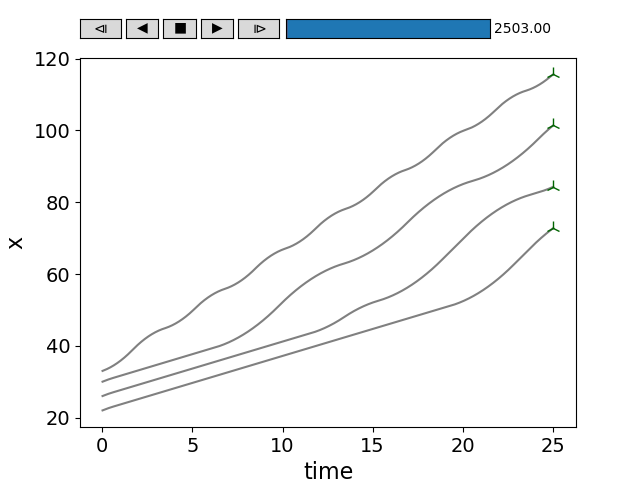
\includegraphics[width=.5\textwidth]{figs/braking_acc.png}\hfill
%\includegraphics[width=.3\textwidth]{figs/Platooning_2.png}}\hfill%
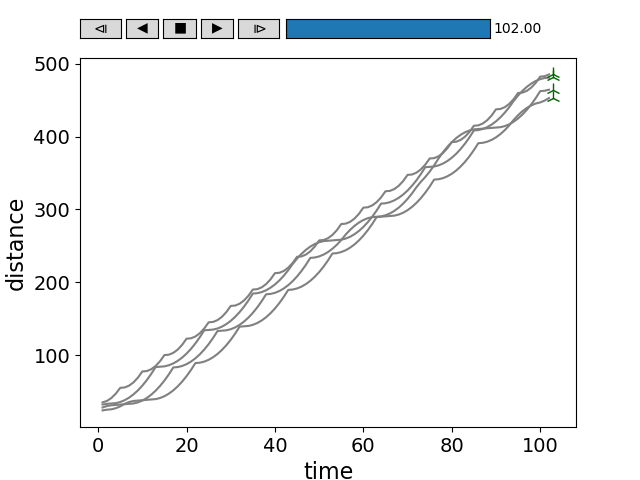
\includegraphics[width=.5\textwidth]{figs/braking_bad.png}
\end{minipage}%
	\caption{\small {Platoon of four cars. \emph{Left} for $\delta = 0.01$, the cars eventually get to safe separations, while reacting to the first car changing its acceleration periodically} and \emph{Right} for $\delta = 0.1$, this shows an unsafe execution where the simulation stops upon a collision.}
\label{fig:platoon}
\end{figure}

%FIGURE OUT THE VERIFICATION. 
% While the simulator enables quick cycles of development and testing, the verification component, as stated earlier, allows the user to tune the conditions under which the program exhibits desired behavior. 
 A \emph{correct} program should ensure that at no point, the separation along the $x$-axis between two of agents is less than the required safe distance ($8$ m).  Note, that the variable $\emph{threshold}$ needs to be set to be higher for larger values of the round duration $\delta$. If $\delta$ is too long, then the cars will not slow down even when the separation between then might have become less than the $\mathit{threshold}$. We verified using the $\kbmc$ tool that \emph{Platoon} is safe for four cars when $\delta$ is small enough and has potential unsafe behaviors otherwise. \reffig{platoon}(Right) shows the $x$ vs $\mathit{time}$ for a counterexample with  $\delta$ is too long. For a threshhold value of $8.0$, required minimum separation of $5.0$, for $\delta = 0.01$ $\kbmc$  showed that the program was safe for 10 rounds starting at an initial configuration where each car $i$ is at a distance of 6.0 from the car $\mathit{i}+1$, For $\delta = 0.1$ $\kbmc$ showed that the program was unsafe. 
 
%\sayan{Last 2 sentences are not clear. What changed between the safe and the unsafe scenarios? Explain clearly. Put a box around the code.}

\subsection{Swarm formation}
%portability
\label{sec:formation}
We used $\lgname$ to implement several standard pattern formation protocols like the  \emph{Lineform} app from the Introduction.  
%
%\begin{figure}[ht!]
%	\label{fig:lineform}
%	\noindent
%	\begin{center}
%		\scriptsize
%		\two{0.4}{0.6}
%		{\lstinputlisting[language=xyzNums,frame=none]{code/lineform.tex}}
%		{ \vspace{0.1in}
%                        $x_{t+1} = Ax_{t}$, where \\
%			$x_0$: vector of initial position of agents, \\
%			$x_{t}$: position vector at time $t$, and \\
%		        $A$: is the \emph{transition matrix}, for lineform  \\
%                  
%			$A  = \left[ \begin{array}{ccccc}
%			0 & 0 & 0 & 0 & 0\\
%			\frac{1}{2} & 0 & \frac{1}{2} & 0 & 0\\
%			0 & \frac{1}{2} & 0 & \frac{1}{2} & 0  \\
%			0 & 0 & \frac{1}{2} & 0 & \frac{1}{2} \\
%			0 & 0 & 0 & 0 & 0\\			
%			\end{array}\right]$
%			}
%	\par
%        
%	\end{center}
%	\caption{\small $\lgname$ program for line formation ({\em Left}) and its mathematical counterpart in robotics and control textbooks ({\em Right}).}
%\end{figure}
%
The shared \emph{allread} variable $x$ is used by the agents to communicate their position to the other robots. The function \emph{mid} computes the centroid of a list of vectors.
% In the case of 3D shape formation,  
%is a part of the library functions provided for the data type \emph{pos}; where 
%$$\mathit{midpoint}(p_1,p_2,\ldots,p_n) = pos(\frac{\Sigma_n p_i.x}{n},\frac{\Sigma_n p_i.y}{n},\frac{\Sigma_n p_i.z}{n}) $$.


With the addition of an explicit neighbor relation, the \emph{Squareform} app as shown in \reffig{squareform} can be used to generate a rhombus shape in the plane formed by four extremal points. The code defines a local variable $nbrs$ which is a static list of list of integers, where the $i$th element is a list of the $\mathit{pid}$s of the neighbors of the agent with $\mathit{pid}$ $i$. The list of $\mathit{pid}$s of the extremal points is stored in a list of integers called $\mathit{corners}$. If the agent $\mathit{pid}$ is not in $\mathit{corners}$, then it moves to the mid point of all its neighbors. \footnote{We omit the actual initialization of the variables $\mathit{nbrs}$ and $\mathit{corner}$, as it depends on the simulation parameters.}

\begin{figure}[ht!]
\begin{mdframed}
    \noindent
    \begin{center}
        \scriptsize
        \two{0.4}{0.6}  {\lstinputlisting[language=koordNums,firstline=1,lastline=10,frame=none]{code/shapeform.tex}}
{\lstinputlisting[language=koordNums,firstline=11,frame=none,firstnumber=11]{code/shapeform.tex}}
    \end{center}
\end{mdframed}
    \caption{$\lgname$ application forming a shape in 3D defined by the static corners.}
    \label{fig:squareform}
\end{figure}

\reffig{shapeplots} shows two screenshots of the 3d-simulation for the \emph{Shapeform} app with 25 agents. Here the $\mathit{Motion}$ controller used is a simple drone model. Instead of the $\mathit{mid}$ function, other operators on the positions of the neighboring agents could be applied to create different swarming protocols. In addition, using the scripting technique for the leading vehicle in $\mathit{Platoon}$, the swarming robots can be guided to move in formation.


\subsection{Distributed task allocation}
\label{sec:task}
 \reffig{taskapp} shows the distributed task allocation application written in $\lgname$. Distributed task allocation is challenging as it involves mutual exclusion as well as construction of de-conflicted paths to task locations. Tasks can be abstractions for real location-based objectives like package delivery, surveillance, or fire-fighting. 

We implement a  task allocation strategy using shared variables for coordination. Mutual exclusion is always an essential feature when shared variables are involved. $\lgname$ provides a locking mechanism using the keyword $\mathit{atomic}$, which the $\mathit{Assign}$ event uses to update the shared list of tasks $\mathit{taskList}$ safely. 

Here the motion module implements Dubin-like vehicle models for the agents, and RRT-based path planning to avoid static obstacles specified in map. \reffig{taskplots} shows two screenshots of a $\mathit{Task}$ application simulations. 

\begin{figure}[h!]
\begin{minipage}{0.5\textwidth}
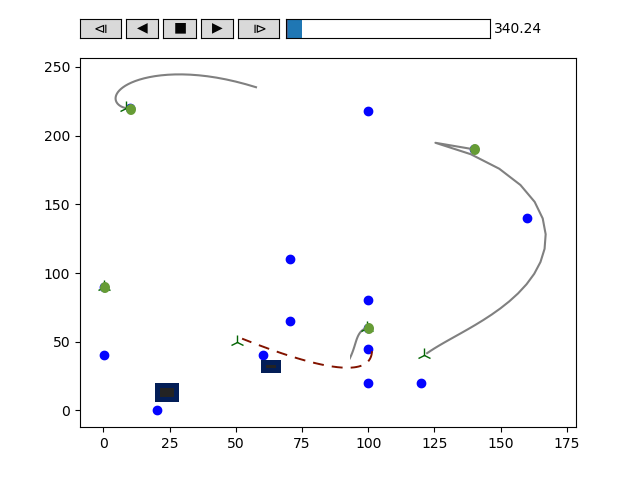
\includegraphics[width=.5\textwidth]{figs/task2.png}\hfill
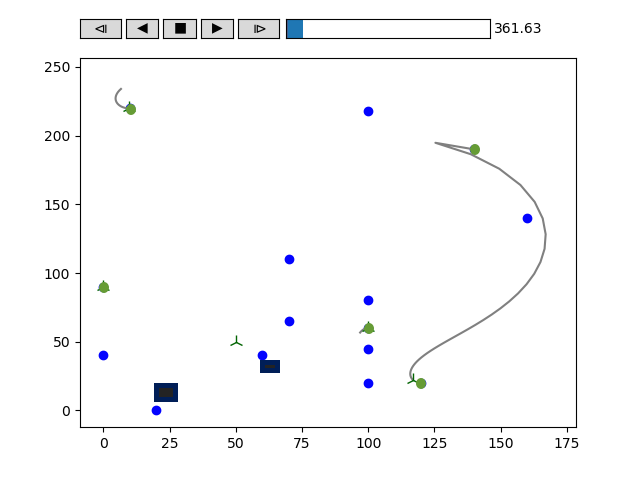
\includegraphics[width=.5\textwidth]{figs/task1.png}\hfill%
%\includegraphics[width=.3\textwidth]{figs/Platooning_2.png}}\hfill%
\end{minipage}%
\caption{\small The grey trails represent the positions of the five agents in the last $150$ time units; task locations of the incomplete tasks (blue), completed tasks (green), static obstacles (black), currently computed infeasible path (dashed red).}
\label{fig:taskplots}
\end{figure}

We could  easily replace the $\mathit{Motion}$ automaton (consequently, the dynamical model) of any of the agents, and run the same code. Using different control parameters, and path planning parameters for the same motion automaton we obtain different statistics for task completion and distance traversal as depicted in in \reffig{completionstats}. This heterogeneity and portability can be useful for coordinating the same application between different hardware platforms. We ran the task application for various configurations of cars (moving in 2d) and quadcopters (moving in 3d) for the task application, and present some completion statistics below. The agents performed 25 tasks, with three obstacles. An agent (car or quadcopter) is considered to have reached a task location if the $x$ and $y$ coordinates of the task are within a specified minimum distance of the current $x$ and $y$ coordinates of the agent.

 For all agents operating with the same motion automaton and dynamics model, we observed that conflict resolution took more time with more agents, as expected (\reffig{completionstats}). The completion time remained relatively stable. The maximum and minimum distances travelled were relatively closer with more robots. However, all these results were affected by the non-determinism in choice of paths and tasks by the agents, and their previous relative positions at the moment of choosing the next task as well. 
 
 
\begin{wrapfigure}{r}{0.26\textwidth}
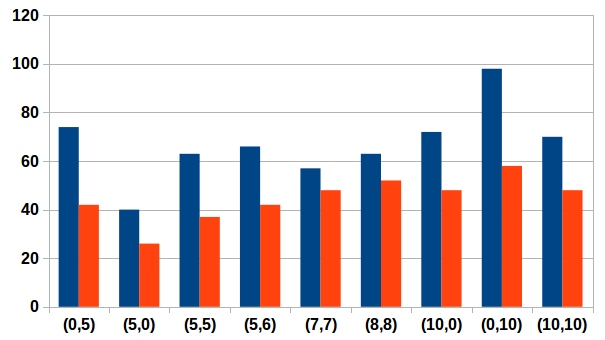
\includegraphics[scale=0.3]{figs/completion.png}\hfill
\caption{\small Completion time (orange) and conflict resolution time (blue)  for different agent configurations (quadcopters, cars). }
\label{fig:completionstats}
\end{wrapfigure}

These results demonstrate a capability of covering various scenarios with different levels of heterogeneity and coordination.
 
